\chapter{Geladenes Teilchen im elektrischen Feld\label{chapter:efeld}}
\lhead{Teilchen im elektrischen Feld}
\begin{refsection}
\chapterauthor{Michael Cerny und Stefan Schindler}


In diesem Kapitel erweitern wir das Beispiel des Potentialkastens 
(Kapitel \ref{subsection:potentialkasten}, Seite \pageref{subsection:potentialkasten})
um eine St\"orung.

\section{St"orungstheorie}
Grunds"atzlich k"onnen wir mit der St\"orungstheorie ein einfaches Modell 
(Abb \ref{abb:efeld_psi_ungestoert} der ersten 5 Energieniveaus) 
mit einer St\"orung erg"anzen, statt von Anfang an mit einem komplexen Modell zu rechnen.

Allgemein gilt:
\[
  f(x, \varepsilon) = f_0(x) + \varepsilon*f_1(x) + \varepsilon^2*f_2(x) + \ldots + \varepsilon^\infty*f_\infty(x)
\]
Dabei ist $f_0(x)$ die urspr\"ungliche Funktion und $f_n(x)$ die $n$-te  N"aherung der St"orung.
Mit $\varepsilon$ wird die St"orung gesteuert. Dabei sollte $\varepsilon$ nicht zu gross gew"ahlt werden, 
da die N"aherung sonst ungenau wird. 

Setzen wir $\varepsilon = 0$, k\"onnen wir die St"orung dynamisch abschalten.

In der Quantenmechanik k"onnen wir die St"orungstheorie anwenden indem wir den Hamilton-Operator der 
urspr"unglichen Funktion $H_0$ um zus"atzliche $\varepsilon^n*H_n$ erg"anzen:
\[
  H = \varepsilon^0*H_0 + \varepsilon^1*H_1 + \varepsilon^2*H_2 + \ldots + \varepsilon^\infty \hat H_\infty
\]












\section{Anwendungen}

\subsection{Potentialkasten mit eFeld}


\subsubsection{Modell der St\"orung elektrisches Feld}

In diesem Modell wollen wir den Grundzustand mit einem elektrischen Feld st\"oren.

Diese St\"orung heisst in der 1. N\"aherung $\hat H_1$ \& wird wie die gesamte St"orung \"uber den 
Parameter $\varepsilon$ gesteuert.

$V_1$ wird als lineares Feld definiert:
\begin{equation}
  V_1(x) = a*x + b
\end{equation}

Der Parameter $a$ steht f\"ur die Feldst\"arke, der Parameter $b$ f\"ur die Grundspannung.

Da wir $a$ jedoch bereits durch $\varepsilon$ beschreiben, k\"onnen wir mit $a = 1$ vereinfachen.

F\"ur die Berechnung ist es einfacher das Feld symetrisch anzulegen. Darum setzen wir $b = 0$ \& reduzieren:
\[
  V_1(x) = x
\]

f\"ur das Potential $V_0(x)$ gilt
\begin{equation}
  \label{eq:efeld_v0_kasten}
  V_0(x)=\begin{cases}
    0       & \qquad |x|<l\\
    \infty  & \qquad\text{sonst.}
  \end{cases}
\end{equation}

Eingesetzt wird daraus:

\[
  \hat{H} = \varepsilon^0 ( \frac{\hbar^2}{2m} \frac{\partial^2}{\partial x^2} + V_0(x) )
            + \varepsilon^1 ( \frac{\hbar^2}{2m} \frac{\partial^2}{\partial x^2} + x )
\]


\begin{figure}
 \centering
 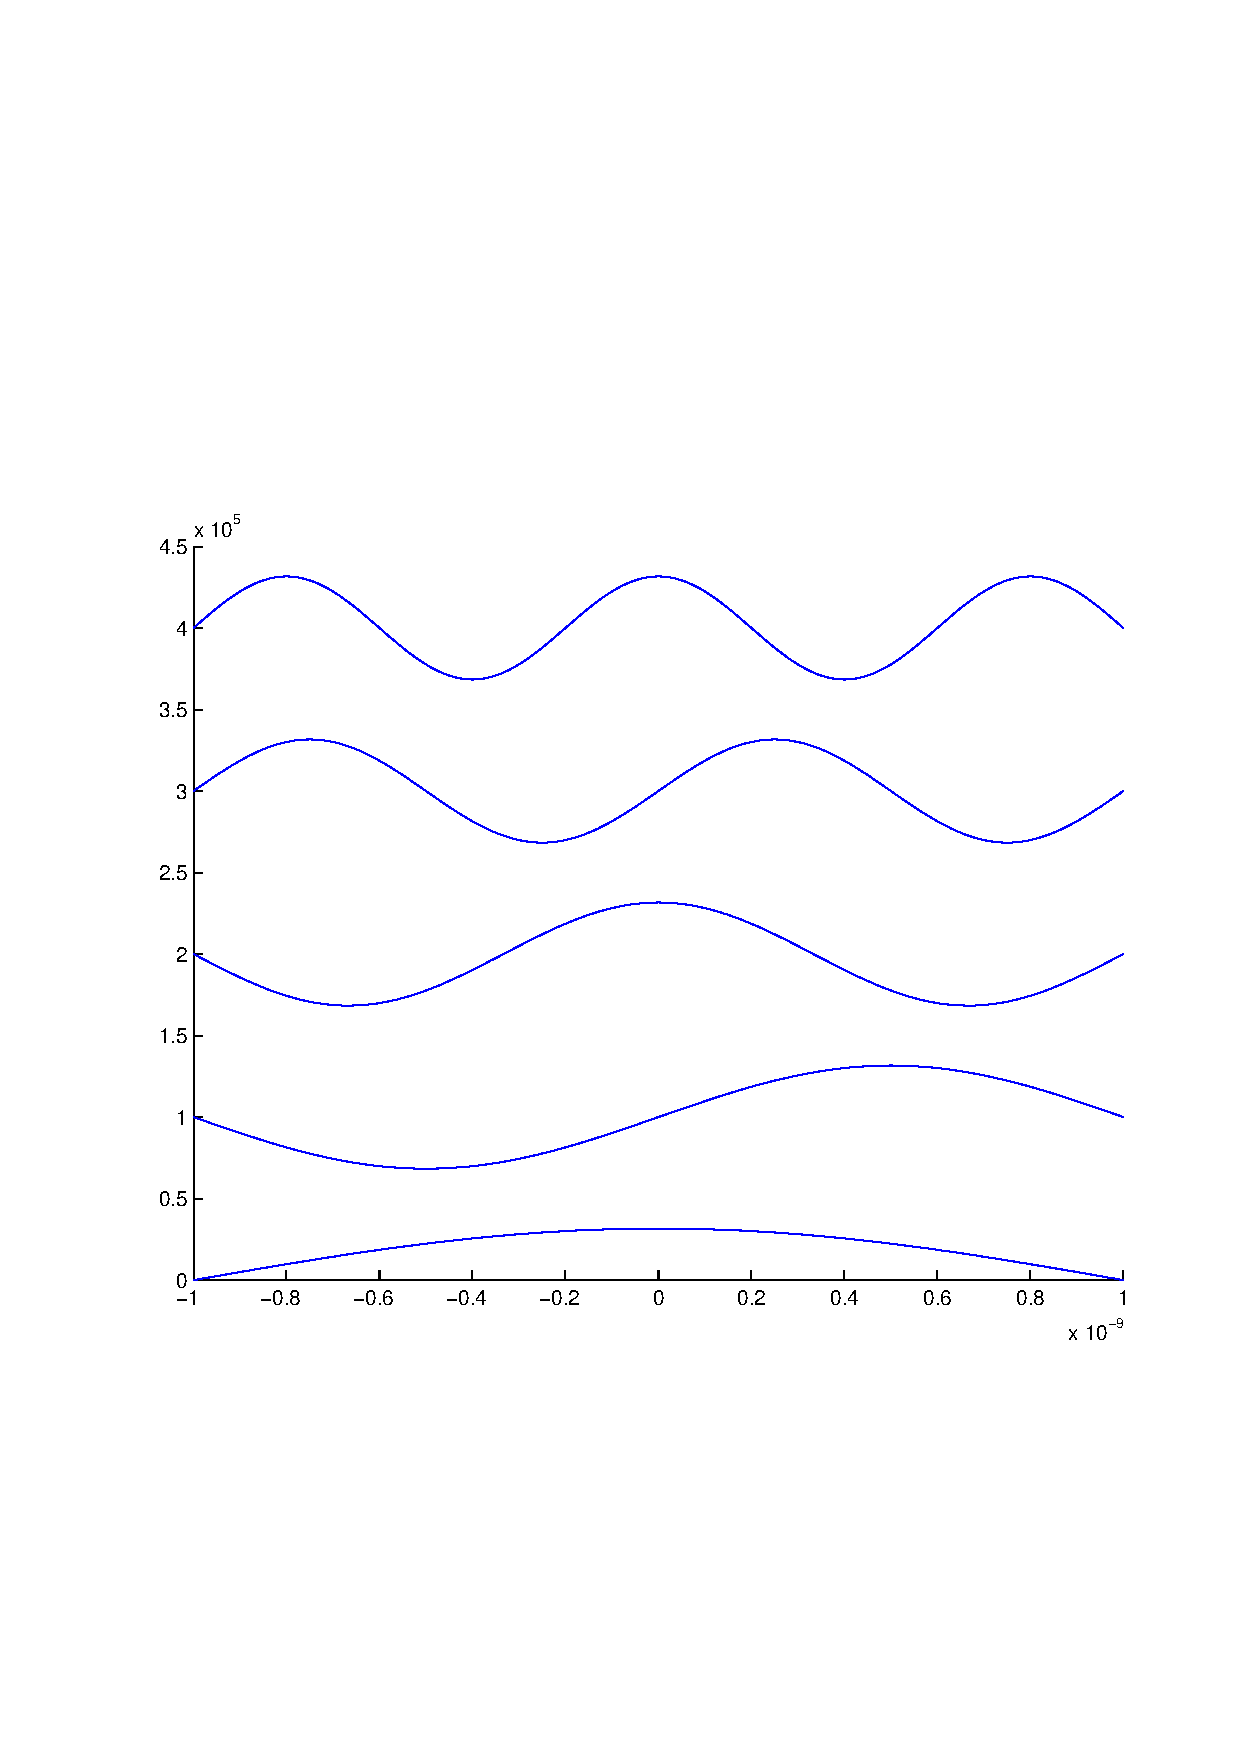
\includegraphics[width=12cm,clip=true,trim=2cm 7cm 1cm 8cm]{efeld/Psi_ungestoert.pdf}
 \caption{$\psi$ ungest\"ort}
 \label{abb:efeld_psi_ungestoert}
\end{figure}








\subsubsection{Berechnung 1. N"aherung}


Wir berechnen in diesem Beispiel die erste N"aherung von einem Potentialskasten mit elektrischem Feld.
Dazu erweitern wir das einfache System  $\hat H_0$
(Siehe Abbildung \ref{skript:potentialkasten})
um $\hat H_1$, welcher die St"orung darstellt.
\[
  \hat{H} = \hat H_0 + \varepsilon \hat H_1
\]

F"ur $\hat H_0$ nehmen wir die Funktion aus dem Skript
\[
  \hat H_0 = \frac{\hbar^2}{2m} \frac{\partial^2}{\partial x^2} + V_0(x)
\]
wobei wir f"ur das Potential $V_0(x)$ die Gleichung \ref{eq:efeld_v0_kasten} nehmen.

Die Ausgangsgleichung f\"ur $\hat{H}$ lautet somit:
\[
  \hat{H} = \varepsilon^0 ( \frac{\hbar^2}{2m} \frac{\partial^2}{\partial x^2} + V_0(x) )
            + \varepsilon^1*x
\]

Ausserdem ist das urspr"unglich $Psi_k^{(0)}$ gegeben.

Um jetzt das gest"orte System zu berechnen brauchen grunds"atzlich nur drei Formeln:
\begin{equation}
\begin{aligned}
k&=l
&&\Rightarrow&
E_k^{(1)}
&=
\langle \psi_k^{(0)}|\, H_1 \,|\psi_k^{(0)}\rangle
\\
k&\ne l
&&\Rightarrow&
\langle\psi_l^{(0)}|\psi_k^{(1)}\rangle
&=
\frac{\langle \psi_l^{(0)}|\, H_1 \,|\psi_k^{(0)}\rangle}{E_k^{(0)}-E_l^{(0)}}
\end{aligned}
\end{equation}
\begin{equation}
|\psi_k(\varepsilon)\rangle
=
(1+i\varepsilon \gamma)
\,|\psi_k^{(0)}\rangle
+
\varepsilon
\sum_{k\ne l}
\frac{\langle \psi_l^{(0)}|\, H_1 \,|\psi_k^{(0)}\rangle}{E_k^{(0)}-E_l^{(0)}}
\,
|\psi_l^{(0)}\rangle
\end{equation}

Mit der ersten Gleichung k"onnen wir direkt die Energie der St"orung berechnen.

Man berechnet also das Skalarprodukt aus $\psi_k^{(0)}$ und $x*\psi_k^{(0)}$ "uber die gesamte L"ange vom Potenzialkasten und erh"alt so $E_k^{(1)}$.

Um jetzt die endg"ultige Energie zu bekommen rechnet man $E_k^{(0)} + \varepsilon*E_k^{(1)}$

Das kann in Matlab einfach geplottet werden mit
\begin{lstlisting}[style=Matlab]
...
H1 = x;
for k = 1 : 5
  E1(k) = dot(Psi(k, :), H1.*Psi(k, :));
  plot(Epsilon, E0(k) + Epsilon*E1_k(k))
end
\end{lstlisting}
In Psi befinden $k$ Vektoren mit diskreten Abtastwerten von $\psi^{(0)}$, die mit Psi(k, :) ausgelesen werden.

Das Resultat sehen wir in der Abbildung \ref{abb:efeld_E_gestoert}.

Um $\psi_k(\varepsilon)$ zu berechnen wird es etwas schwieriger, weil sich in der Quantenmechanik die Energiezust"ande $k$ gegenseitig beeinflussen.

Daher setzen wir eine St"orung $\psi_k^{(1)}$ aus mehreren $\psi_k^{(0)}$ zusammen.
Mit der zweiten und dritten Formel k"onnen wir diesen Anteil berechnen.

\begin{equation}
  \label{eq:efeld_skalar_gleichung}
  \langle\psi_l^{(0)}|\psi_k^{(1)}\rangle
      =
  \frac{\langle \psi_l^{(0)}|\, H_1 \,|\psi_k^{(0)}\rangle}{E_k^{(0)}-E_l^{(0)}}
\end{equation}

Die Formel \ref{eq:efeld_skalar_gleichung} gibt uns einen Skalarwert, welcher uns zeigt wie viel Anteil die Welle $l$ an der St"orung $k$ hat.

Um zum Beispiel den f"unften Zustand $\psi_5^{(1)}$ zu bestimmen addieren wir alle 
$\langle\psi_l^{(0)}|\psi_5^{(1)}\rangle*|\psi_l^{(0)}\rangle$
 von 1 bis $\infty$ ausser 5.
\begin{equation}
  \sum_{l=1 ; l\ne 5}^{\infty}
    \frac{\langle \psi_l^{(0)}|\, H_1 \,|\psi_k^{(0)}\rangle}{E_k^{(0)}-E_l^{(0)}}
        \,
    |\psi_l^{(0)}\rangle
\end{equation}

In Matlab kann man das mit folgendem Code berechnen:
\begin{lstlisting}[style=Matlab]
...
x = -10^-9 : delta : 10^-9;
H1 = x;
n = 1000;
k = 5;
summe = 0;
for l = 1 : n
  if l ~= k
    Psi0_l = dot(Psi(l, :), H1.*Psi(k, :)) / (E(k)-E(l)) .* Psi(l, :);
    summe = psi1_l + psi0_l;
  end
end
\end{lstlisting}

Man muss $n$ zum Gl"uck nicht auf unendlich setzen, da der Anteil durch den Term $\frac{1}{E(k)-E(l)}$ immer weiter abnimmt.
In diesem Fall addieren wir bei $l=90$ nur 1\% der St"orung dazu, bei $l=280$ nur noch $0.1\%$.

Wir k"onnen jetzt die St"orung in 
\begin{equation}
|\psi_k(\varepsilon)\rangle
=
(1+i\varepsilon \gamma)
\,|\psi_k^{(0)}\rangle
+
\varepsilon*|\psi_k^{(1)}\rangle
\end{equation}
einsetzen und bekommen so die neue Wellenfunktion die man in \ref{abb:efeld_psi_gestoert} sehen kann.

In der Grafik \ref{abb:efeld_psi_gestoert} sehen wir die Unterschiede zwischen dem normalen $\psi$ (schwarz) \& der ersten N"aherung (rot).

In diesem Beispiel haben wir die Unterschiede mit sehr starken Parametern gew"ahlt.

Die einzelnen Werte in y-Richtung sind die jeweiligen N"aherungen. Alle Kurven pendeln um die x-Achse.

\begin{figure}
 \centering
 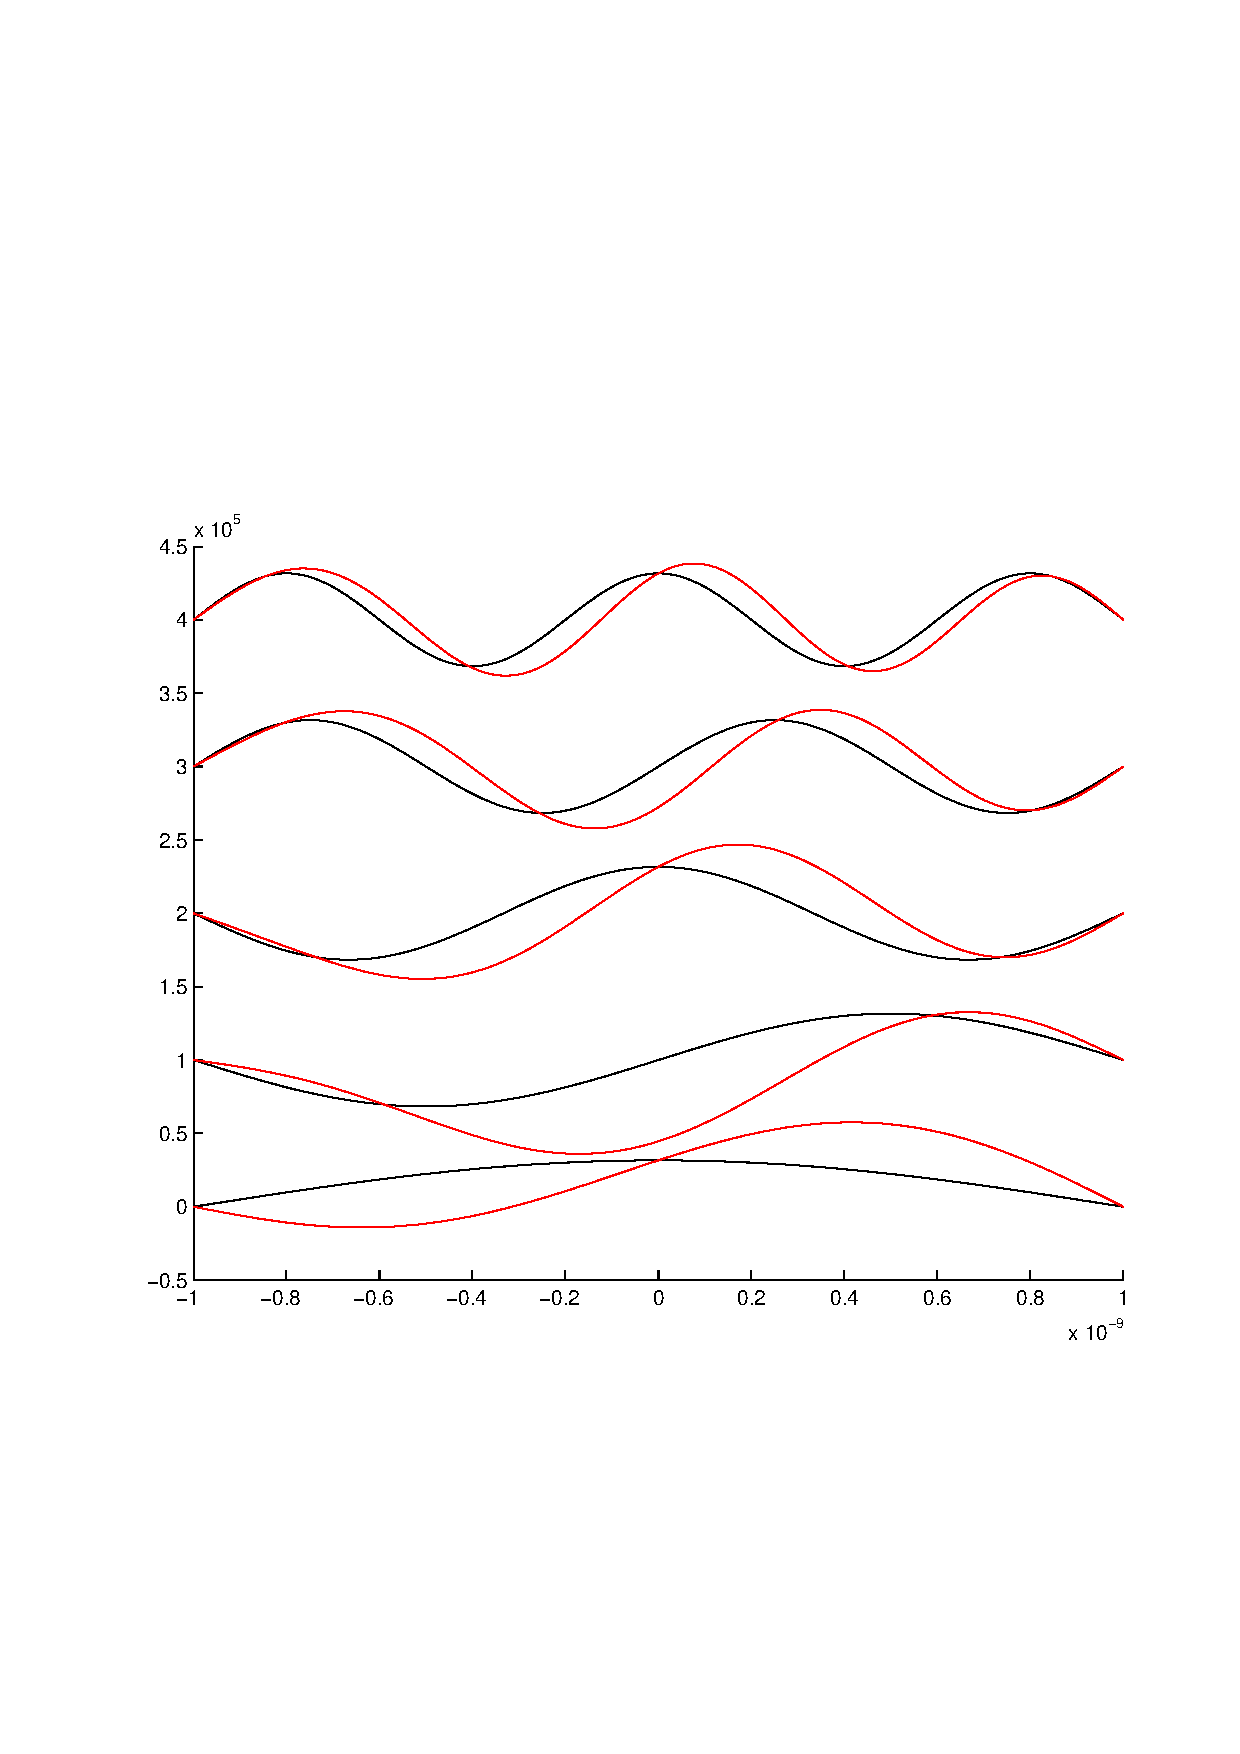
\includegraphics[width=12cm,clip=true,trim=2cm 7cm 1cm 8cm]{efeld/Psi_gestoert.pdf}
 \caption{$\psi$ gest\"ort}
 \label{abb:efeld_psi_gestoert}
\end{figure}




\subsubsection{Energie "Anderung}

Was passiert?

In der Grafik \ref{abb:efeld_E_gestoert} lassen wir f"ur die jeweiligen stabilen Zust"ande 0..4 
den Einfluss der St"orung wachsen.

Da das elektrische Feld jedoch nur einen sehr kleinen Einfluss auf die gesammte Energie des 
Elektrons hat, mussten wir um die Effekte der 1. N"aherung zu zeigen ein sehr grosses $\varepsilon$
w"ahlen.

\begin{figure}
 \centering
 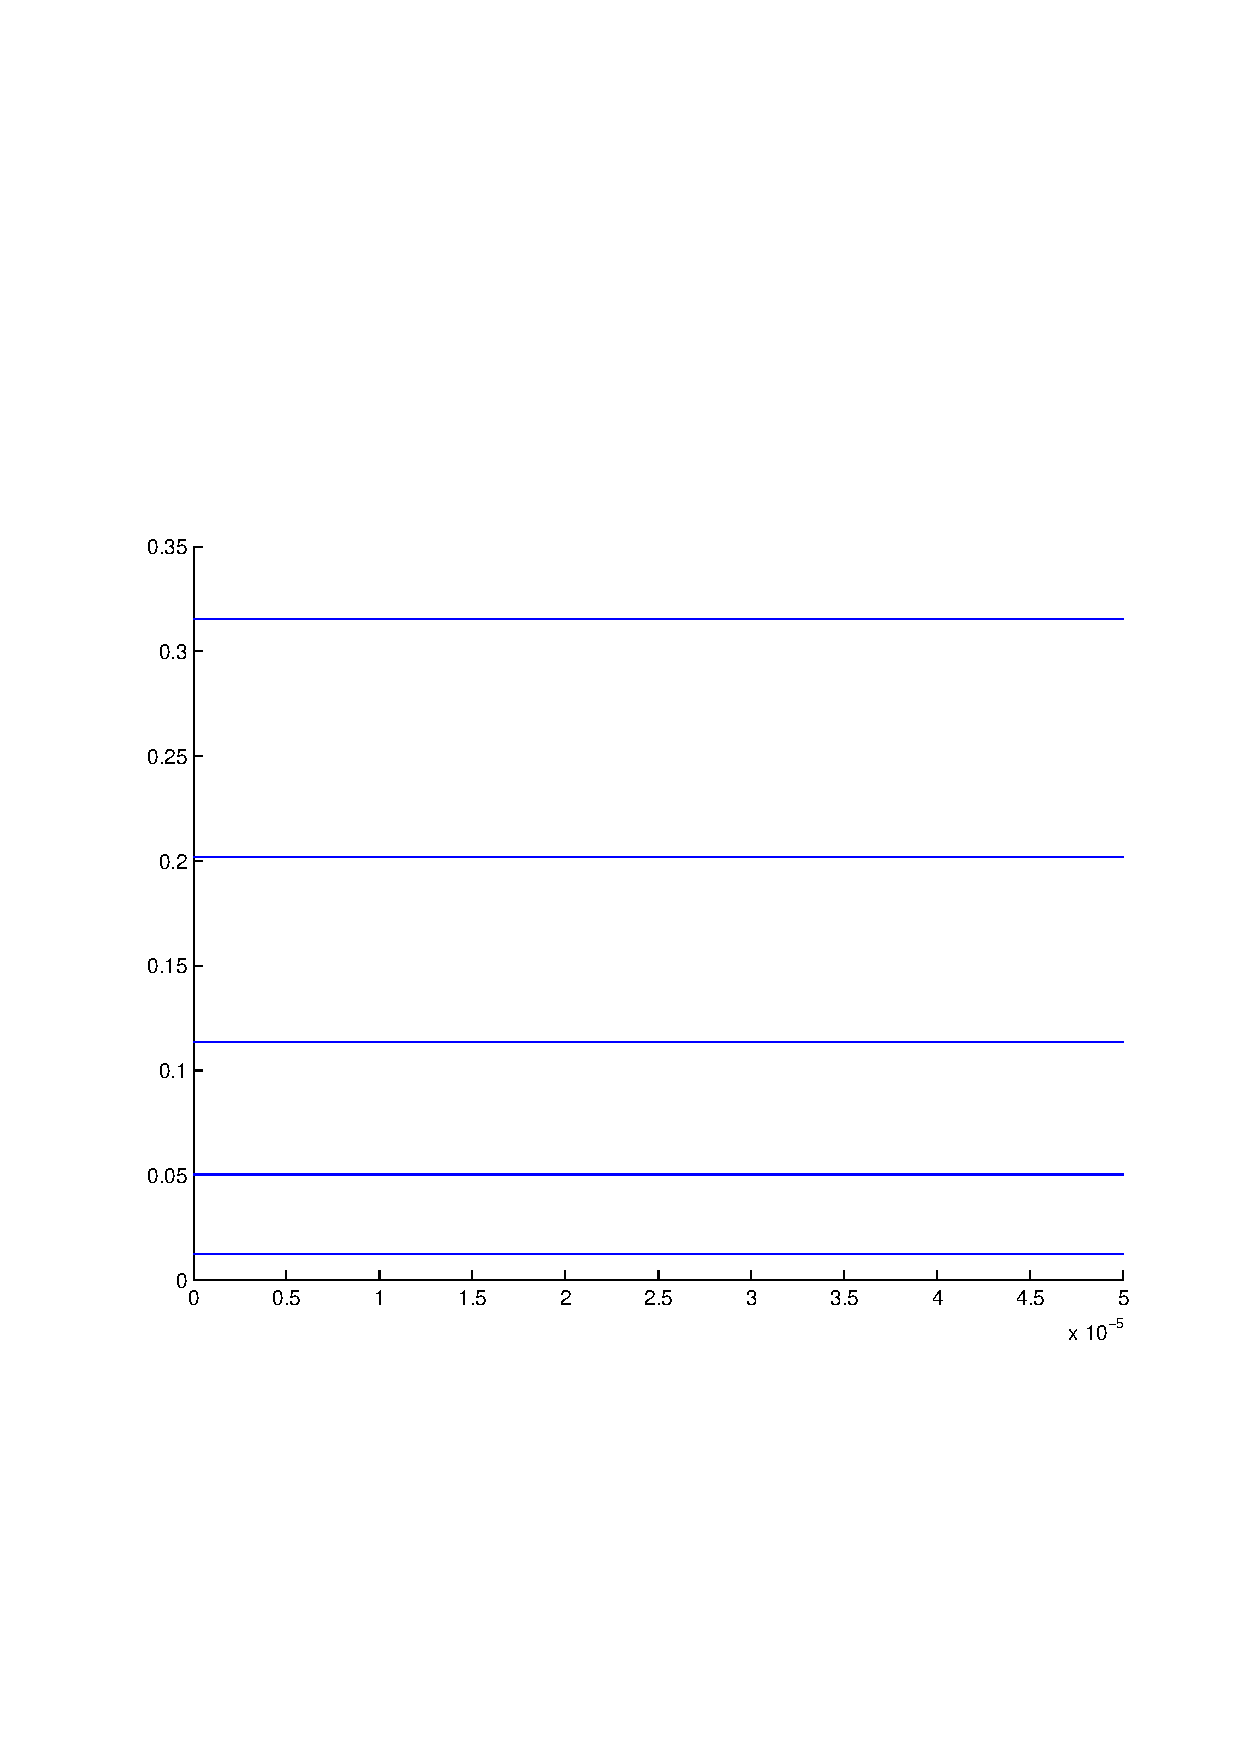
\includegraphics[width=12cm,clip=true,trim=2cm 7cm 1cm 8cm]{efeld/Energie_gestoert.pdf}
 \caption{$E$ gest\"ort, x-Achse ist $\varepsilon$, y-Achse ist die gesammte Energie des Systems}
 \label{abb:efeld_E_gestoert}
\end{figure}











\subsection{Potentialtopf}

In dieser Anwendung definieren wir das Potential ausserhalb von $l$ nicht mehr mit $\infty$, das Elektron kann mit gen"ugend Energie aus dem Topf gehoben werden.

\subsubsection{Berechnung 1. N"aherung}

Wir definieren den Potentialtopf basierend auf der Formel \ref{eq:efeld_v0_kasten}:
\begin{equation}
  V_0(x)=\begin{cases}
    0       & \qquad |x|<l\\
    1  & \qquad\text{sonst.}
  \end{cases}
\end{equation}

Wir "ubernehmen die St"orung aus der ersten Anwendung.
\[
  V_1 = x
\]


\printbibliography[heading=subbibliography]
\end{refsection}
